\documentclass[twoside]{article} \usepackage{aistats2017}

% If your paper is accepted, change the options for the package
% aistats2017 as follows:
%
%\usepackage[accepted]{aistats2017}
%
% This option will print headings for the title of your paper and
% headings for the authors names, plus a copyright note at the end of
% the first column of the first page.
\usepackage{amsmath,amsthm,color,graphicx,verbatim,listings,enumitem,float}
\usepackage{amssymb}
\usepackage{natbib}  % for references
\usepackage{amsfonts}
\usepackage{nicefrac}  
\usepackage{booktabs}
\usepackage{microtype}
\usepackage[]{algorithm2e}
\usepackage{caption}
\usepackage{subcaption}
\graphicspath{{figures/}}
\usepackage{setspace}
\lstset{
numbers=left, 
numberstyle=\small, 
numbersep=8pt, 
frame = single, 
language=matlab, 
framexleftmargin=20pt}

\renewcommand{\refname}{}
\newcommand{\simiid}{\overset{\textrm{i.i.d.}}{\sim}}
\DeclareMathOperator*{\argmin}{arg\,min}
\newtheorem{lemma}{Lemma}
\newtheorem{theorem}{Theorem}
\newtheorem{corollary}{Corollary}

% This portion of style definition will remove the index number before the 
% without inducing an indent
\makeatletter
\renewcommand\@biblabel[1]{}
\renewenvironment{thebibliography}[1]
     {\section*{\refname}%
      \@mkboth{\MakeUppercase\refname}{\MakeUppercase\refname}%
      \list{}%
           {\leftmargin0pt
            \@openbib@code
            \usecounter{enumiv}}%
      \sloppy
      \clubpenalty4000
      \@clubpenalty \clubpenalty
      \widowpenalty4000%
      \sfcode`\.\@m}
     {\def\@noitemerr
       {\@latex@warning{Empty `thebibliography' environment}}%
      \endlist}
\makeatother

\begin{document}

% If your paper is accepted and the title of your paper is very long,
% the style will print as headings an error message. Use the following
% command to supply a shorter title of your paper so that it can be
% used as headings.
%
%\runningtitle{I use this title instead because the last one was very long}

% If your paper is accepted and the number of authors is large, the
% style will print as headings an error message. Use the following
% command to supply a shorter version of the authors names so that
% they can be used as headings (for example, use only the surnames)
%
%\runningauthor{Surname 1, Surname 2, Surname 3, ...., Surname n}

\twocolumn[

\aistatstitle{An Efficient Minibatch Acceptance Test for Metropolis-Hastings}

\aistatsauthor{ Anonymous Author 1 \And Anonymous Author 2 \And Anonymous Author 3 }

\aistatsaddress{ Unknown Institution 1 \And Unknown Institution 2 \And Unknown Institution 3 } ]

\begin{abstract}
  %The Abstract paragraph should be indented 0.25 inch (1.5 picas) on
  %both left and right-hand margins. Use 10~point type, with a vertical
  %spacing of 11~points. The {\bf Abstract} heading must be centered,
  %bold, and in point size 12. Two line spaces precede the
  %Abstract. The Abstract must be limited to one paragraph.
  Markov chain Monte Carlo (MCMC) methods have many applications in
  machine learning. We are particularly interested in their application
  to modeling very large datasets, where it is impractical to perform
  Metropolis-Hastings tests on the full data. Previous work on reducing
  the cost of Metropolis-Hastings tests yield variable data consumed per
  sample, with only constant factor reductions versus using the full
  dataset for each sample.  Here we present a method that can be tuned
  to provide arbitrarily small batch sizes, by adjusting either proposal
  step size or temperature. Our approach uses the natural noise present
  in minibatch likelihood estimates to furnish the randomness in a
  Metropolis-Hastings test. Our test uses the noise-tolerant Barker
  acceptance test with a novel additive correction variable.  The
  resulting test can be combined with minibatch proposals to yield
  updates with the same complexity as a simple SGD update. In this paper
  we derive the test, analyze its performance, discuss its
  implementation, and present several experiments. We demonstrate 
  several order-of-magnitude speedup over previous work, and show for
  the first time that small expected minibatch sizes are possible. 
\end{abstract}

\section{INTRODUCTION}\label{sec:introduction}

Markov chain Monte Carlo (MCMC) sampling is a powerful method for computation on
intractable distributions. We are interested in large dataset applications,
where the goal is to sample a posterior distribution $p(\theta \mid x_1, \ldots,
x_N)$ of parameter $\theta$ for large $N$.  The Metropolis-Hastings method (M-H)
generates sample candidates from a proposal distribution $q$ which is in general
different from the target distribution $p$, and decides whether to accept or
reject based on an acceptance test. The acceptance test is usually a Metropolis
test~\citep{Metropolis1953, hastings70}.

Many state-of-the-art machine learning methods, and deep learning in particular,
are based on minibatch updates (such as SGD) to a model.  Minibatch updates
produce many improvements to the model for each pass over the dataset, and have
high sample efficiency.  In contrast, conventional M-H requires calculations
over the full dataset to produce a new sample.  Recent results
from~\citet{cutting_mh_2014} and~\citet{icml2014c1_bardenet14} perform
approximate (bounded error) acceptance tests using subsets of the full dataset.
The tests depend on minibatch statistics, and on the value of an additional
uniform random variable $u$. The amount of data consumed for each test varies
significantly from one minibatch to the next, and depends on the current sample,
the proposed sample, and on the random variable $u$. By
contrast,~\citet{conf/uai/MaclaurinA14,TallData15} perform exact tests but
require a lower bound on parameter distribution across its domain.  The amount
of data reduction depends on the accuracy of this bound, and such bounds are
only available for relatively simple distributions.


Here we derive a new test which incorporates the variability in minibatch
statistics as {\em a natural part of the test} and requires less data per
iteration than prior work. We use a Barker test function~\citep{Barker65}, which
makes our test naturally error tolerant. The idea of using a noise-tolerant
Barker's test function was suggested but not explored empirically
in~\citet{TallData15} section 6.3. But the asymptotic test statistic CDF and the
Barker function are different, which leads to fixed errors for the approach
in~\citet{TallData15}. Here, we show that the difference between the
distributions can be corrected with an additive random variable. This leads to a
test which is fast, and whose error can be made arbitrarily small.

Our test is applicable when the variance (over data samples) of the log
acceptance probability is small enough (less than 1). It's not clear at first why
this quantity should be bounded, but we will show that it is ``natural'' for
well-specified models running Metropolis-Hastings sampling with optimal
proposals~\citep{OptimalScaling01} on a full dataset. When we reduce the amount
of data for the test, the variance goes up. We have to reduce variance in one
of several ways. Either:

\begin{itemize}[noitemsep]
    \item Increase the temperature of the target distribution. Log likelihoods
    scale as $1/T$, and so the variance of the likelihood ratio will vary as
    $1/T^2$. Our model is no longer well-specified (we are doing inference at a
    temperature different from that assumed during data generation), but higher
    temperature can be advantageous for parameter exploration.

    \item For continuous probability distributions, reduce the proposal step
    size and variance (for stochastic proposals) compared to an optimal
    proposal. The variance of the log acceptance probability scales as the
    square of proposal step size. 

    \item Increase the minibatch size when needed for certain minibatches. Log
    acceptance variance scales as $1/k$ vs the minibatch size $k$. Our test is
    adaptive like earlier works, but unlike them, the distribution of minibatch
    size is Gaussian, not long-tailed.  Increased minibatch size also reduces
    the error rate for the test.
\end{itemize}

It is worth discussing at this point the typical goals of M-H sampling on large
datasets.  By the Bernstein-von Mises Theorem, the posterior distribution for a
Bayesian inference task is asymptotically normal, and has variance that scales
inversely with the $N$ data samples. Simply sampling from this distribution is
one application, but an efficient proposal~\citep{OptimalScaling01} has similar
variance to the target distribution and will diffuse to it extremely slowly from
an initialization value which is (likely to be) many standard deviations away.
If there are any other strong modes, it is very likely for the sampler to find
one of them and become trapped in it when run at the normal distribution
temperature ($T=1$). A common solution is to anneal the sampler, running first
at high temperature (scaling log likelihoods by $1/T$) which flattens the
likelihood landscape.  This in turn reduces the variance of the log acceptance
probability and allows our acceptance test to be applied.

A second question concerns step size. Once we have fixed temperature, our
variance constraint implies that we have to trade-off proposal step size $s$ and
batch size $b$ ($b \propto p^2$), i.e. we can make many small steps, or one
large step, with a given batch of data. One of the primary drivers of this work
is our belief in the value of small steps. For applications to neural networks
or other models where the posterior is multimodal, posterior inference is
arguably a search process. Covering the search space densely with small steps is
much more valuable than few sparse steps toward the nearest optimum. In this
mode, Metropolis-Hastings can be used in similar fashion to Stochastic Gradient
Descent. The goal in SGD is to make gradual progress to a posterior mode with
each step, taking small steps so that the cumulative displacement has
progressively lower variance. We demonstrate this behavior in our logistic
regression experiments. 

The contributions of this paper are as follows:

\begin{itemize}[noitemsep]
    \item We develop a new, more efficient (in samples per test) minibatch
    acceptance test with quantifiable error bounds. The test uses a novel
    additive correction variable to implement a Barker test based on minibatch
    mean and variance. 

    %\item We analyze the test for accuracy and speed.

    \item We compare performance of our new test and prior approaches on several
    datasets. We demonstrate the test is several orders of magnitude more
    efficient than prior work measured as data consumed per test, and that it
    does not suffer from long-tailed minibatch sizes (up to the dataset size). 
\end{itemize}



\section{PRELIMINARIES}\label{sec:related_work}

In the Metropolis-Hastings method~\citep{gilks1996markov,brooks2011handbook}, a
difficult-to-compute probability distribution $p(\theta)$ is sampled using a
Markov chain $\theta_1,\ldots,\theta_n$. The sample $\theta_{t+1}$ at time $t+1$
is generated using a candidate $\theta'$ from a (simpler) proposal distribution
$q(\theta'\mid \theta_t)$, filtered by an acceptance test. The acceptance test
is usually a Metropolis test. The Metropolis test has acceptance probability:
\begin{equation}\label{eq:traditional}
    \alpha(\theta_t,\theta') = \frac{p(\theta')q(\theta_t \mid \theta')}{p(\theta_t)q(\theta' \mid \theta_t)} \wedge 1
\end{equation}
where $a \wedge b$ denotes $\min(a,b)$.  With probability
$\alpha(\theta_t,\theta')$, we accept $\theta'$ and set $\theta_{t+1} =
\theta'$, otherwise set $\theta_{t+1}=\theta_t$.  The test is often implemented
with an auxiliary random variable $u \sim \mathcal{U}(0,1)$ with a comparison
$u<\alpha(\theta_t,\theta')$; here, $\mathcal{U}(a,b)$ denotes the uniform
distribution on the interval $[a,b]$.  For simplicity, we drop the subscript $t$
for the current sample $\theta_t$ and denote it as $\theta$. 

The acceptance test guarantees detailed balance, which means
$p(\theta)p(\theta'\mid\theta) = p(\theta')p(\theta \mid\theta')$,
where $p(\theta'\mid\theta)$ is the probability of a transition from state
$\theta$ to $\theta'$. Here $p(\theta'\mid\theta) =
q(\theta'\mid\theta)\alpha(\theta,\theta')$ so the detailed balance equation
becomes 
\begin{equation}\label{eq:detailed_balance2}
    p(\theta)q(\theta'\mid\theta)\alpha(\theta,\theta') = p(\theta')q(\theta\mid\theta')\alpha(\theta',\theta)
\end{equation}
This condition, together with ergodicity, guarantees that the Markov chain has a
unique stationary distribution $\pi(\theta) = p(\theta)$. For Bayesian inference, we would like to sample from a parameter distribution for $\theta$ based on some observed data, so the target distribution is
$p(\theta \mid x_1, \ldots, x_N)$. The acceptance probability is now:
\begin{equation}\label{eq:acceptance_probability}
    \alpha(\theta,\theta') = 
    \frac{p_0(\theta')\prod_{i=1}^N p(x_i \mid \theta')q(\theta \mid
    \theta')}{p_0(\theta)\prod_{i=1}^N p(x_i \mid \theta)q(\theta' \mid\theta)}
    \wedge 1
\end{equation}
where $p_0(\theta)$ is a prior, and $p(x_i \mid \theta)$ are the probabilities
of the observations. Computing samples this way requires the use of all $N$
training data points, but this is very expensive for large datasets. To address
this challenge,~\citet{cutting_mh_2014,icml2014c1_bardenet14} perform approximate
Metropolis-Hasting tests using sequential hypothesis testing. During each
iteration, they start with a small minibatch of data and test whether the sample $\theta'$ 
should be accepted based on an approximate version of
the test $u < \alpha(\theta,\theta')$. If the approximate test cannot make a
decision with sufficient confidence, then the minibatch size is increased and
the test repeats. This process continues until a decision. The bounds depend on
either an asymptotic Central Limit Theorem~\citep{cutting_mh_2014} or a
concentration bound~\citep{icml2014c1_bardenet14}. The latter requires direct
bounds on the log likelihood ratio, which for general distributions requires
knowing $p(x_i \mid \theta)$ and $p(x_i \mid \theta')$ for all $N$ samples. In
addition, both methods suffer the drawback of resolving small log likelihood
ratio differences between the minibatch and full batch versions.  In the worst
case, all $N$ data points may be needed, as we show in
Section~\ref{ssec:gaussian_example}.

Following~\citet{icml2014c1_bardenet14}, we write the test
$u<\alpha(\theta,\theta')$ in the equivalent form $\Lambda(\theta,\theta') >
\psi(u,\theta,\theta')$, where\footnote{Our definitions differ from those
in~\citet{icml2014c1_bardenet14} by a factor of $N$ to simplify our analysis
later.}
\begin{equation}
\begin{split} 
\Lambda(\theta,\theta') & = \sum_{i=1}^N \log\left(\frac{p(x_i|\theta')}{p(x_i|\theta)}\right) \\  
{\rm and} \quad \psi(u,\theta,\theta') &= \log\left(u\frac{q(\theta'|\theta)p_0(\theta)}{q(\theta|\theta')p_0(\theta')}\right) \\
\end{split}
\end{equation}
To reduce computational effort, an unbiased estimate of $\Lambda(\theta,\theta')$
based on a minibatch can be used:
\begin{equation}
\Lambda^*(\theta,\theta') = \frac{N}{b}\sum_{i=1}^b \log\left(\frac{p(x_i|\theta')}{p(x_i|\theta)}\right)  
\end{equation}
Finally, it will be convenient for our analysis to define the individual
components that contribute to the sums above:
\begin{equation}\label{eq:individual_terms}
\Lambda_i(\theta,\theta') = N \log\left(\frac{p(x_i|\theta')}{p(x_i|\theta)}\right)  
\end{equation}
%Thus, $\Lambda(\theta,\theta')$ is the mean of $\Lambda_i(\theta,\theta')$ over
%the entire dataset, and $\Lambda^*(\theta,\theta')$ is the mean of
%$\Lambda_i(\theta,\theta')$ over its minibatch. 

Since minibatches contains randomly selected samples $x_i$, the values
$\Lambda_i$ are independent, identically distributed (iid) random
variables\footnote{The analysis assumes sampling with replacement
although implementations on typical large datasets will approximate
this by sampling without replacement.}.
By the Central Limit Theorem, we expect $\Lambda^*(\theta,\theta')$ to
be approximately Gaussian. The acceptance test then becomes a
statistical test of the hypothesis that
$\Lambda(\theta,\theta')>\psi(u,\theta,\theta')$ by establishing that
$\Lambda^*(\theta,\theta')$ is substantially larger than
$\psi(u,\theta,\theta')$.  In~\citet{cutting_mh_2014} an asymptotic
central limit argument was used to derive this gap, while
in~\citet{icml2014c1_bardenet14} a concentration bound was used. In
both cases, the resulting tests were shown to give useful reductions
in number of samples required over using the full dataset, but there
were no worst-case bounds given on the average number of samples
needed per iteration, which we explore in the following section.

\subsection{A Worst-Case Gaussian Example}\label{ssec:gaussian_example}
Consider a Gaussian model where $x_1,\ldots,x_N \simiid \mathcal{N}(\theta,1)$
with a known variance $\sigma^2=1$, true mean $\theta=0.5$, and a uniform prior
on $\theta$. The log likelihood ratio is
\begin{equation}\label{eq:lemma_ll_ratio}
    \Lambda^*(\theta,\theta') = N(\theta'-\theta)\left(\frac{1}{b}\sum_{i=1}^b x_i-\theta-\frac{\theta'-\theta}{2}\right)
\end{equation}
which is normally distributed over selection of the Normal samples $x_i$.  Since
the $x_i$ have unit variance, their mean has variance $1/b$, and the variance of
$\Lambda^*(\theta,\theta')$ is $\sigma^2(\Lambda^*) = (\theta'-\theta)^2N^2/b$.
In order to pass a hypothesis test that $\Lambda > \psi$, there needs to be a
large enough gap (several $\sigma(\Lambda^*)$) between
$\Lambda^*(\theta,\theta')$ and $\psi(u,\theta,\theta')$. 

Our goal is to sample from the posterior $p(\theta \mid x_1,\ldots,x_N)$, which
is a normal distribution $\mathcal{N}(\mu, 1/N)$ centered on the sample mean
$\mu$, and with variance $1/N$. In one dimension, an efficient proposal
distribution has the same variance as the target
distribution~\citep{OptimalScaling01}, so we use the proposal
$\mathcal{N}(\theta,1/N)$, which is implemented as
$q(\theta'\mid\theta)=\phi((\theta'-\theta)N)$, where $\phi(x)$ is the Normal
density function with zero mean and unit variance. This proposal is symmetric
$q(\theta'\mid\theta)=q(\theta\mid\theta')$, and since we assumed a uniform
prior on $\theta$, we see that $\psi(u,\theta,\theta')$ reduces to $\log u$. Our
worst-case scenario is specified in Lemma~\ref{lem:worst_case}.

\begin{lemma}\label{lem:worst_case}
    For the model in Section~\ref{ssec:gaussian_example}, there exists a fixed
    (independent of $N$) constant $c$ such that with probability $\geq c$ over
    the joint distribution of $(\theta, \theta', u)$, the tests
    from~\cite{cutting_mh_2014,icml2014c1_bardenet14} consume all $N$ samples. 
\end{lemma}
\vspace{-1em}
\begin{proof}
See Appendix~\ref{app:worst_case_proof}.
\end{proof}
Similar results can be shown for other distributions and proposals by
identifying regions in product space $(\theta,\theta',u)$ such that the
hypothesis test needs to separate nearly-equal values.  It follows that the
accelerated M-H tests in~\citet{cutting_mh_2014,icml2014c1_bardenet14} require at
least a constant fraction $\geq c$ in the amount of data consumed per test
compared to full-dataset tests, so their speed-up is at most $1/c$.

% {\color{blue} Daniel: quick question: I think we should explain why our method
% \emph{doesn't} run into this issue. I think it is because we rely on an
% approximation to $\Delta + X_{\rm log} > 0$ and that test does not require any
% ``difference between an approximation and an exact version'' because it is
% \emph{already} an exact version, assuming the approximation is enough.
% Also, in terms of this example, if we are in the special case with using a lot
% of data, why not force early stopping?}

The problem is that these methods use tail bounds to separate $\Delta$ away
from zero, but for certain input/random $u$ combinations, $\Delta$ can be
arbitrarily close to zero. We will avoid this by using the {\em approximately
normal} variation in $\Delta^*$ to {\em replace} the variation due to $u$. 

\subsection{MCMC Posterior Inference}
There is a separate line of MCMC work drawing principles from statistical
physics. By viewing random variables as particles in a system, one can apply
Hamiltonian Monte Carlo (HMC)~\citep{mcmc_hamiltonian_2010} methods which
generate high acceptance \emph{and} distant proposals when run on full batches
of data. Recently Langevin Dynamics~\citep{langevin_2011,conf/icml/AhnBW12} has
been applied to Bayesian estimation on minibatches of data. This simplified
dynamics uses local proposals and avoids MH tests by using small proposal steps
whose acceptance approaches 1 in the limit. However, the constraint on proposal
step size is severe, and the state space exploration reduces to a random walk.
Full minibatch HMC for minibatches was described in~\citet{sghmc_2014} which
allows momentum-augmented proposals with larger step sizes. However, step sizes
are still limited by the need to run accurately without MH tests.  By providing
an M-H test with similar cost to standard gradient steps, our work opens the
door to applying those methods with much more aggressive step sizes without loss
of accuracy. 




\section{A NEW MH ACCEPTANCE TEST}\label{sec:our_algorithm}

\subsection{Log-Likelihood Ratios}\label{ssec:log_likelihood_ratios}

For our new M-H test, we denote the exact and approximate log likelihood ratios
as $\Delta$ and $\Delta^*$, respectively. First, $\Delta$ is defined as
\begin{equation}\label{eq:delta1}
    \Delta(\theta,\theta')  =
    \log \frac{p_0(\theta')\prod_{i=1}^N p(x_i \mid \theta')q(\theta \mid
    \theta')}{p_0(\theta)\prod_{i=1}^N p(x_i \mid \theta)q(\theta' \mid\theta)},
\end{equation}
where $p_0, p$, and $q$ match the corresponding functions within
Equation~(\ref{eq:acceptance_probability}). We separate out terms dependent and
independent of the data $x$ as:
\begin{equation}\label{eq:delta2}
\begin{split}
    \Delta(\theta,\theta') &= \sum_{i=1}^N\log\frac{p(x_i\mid\theta')}{p(x_i\mid\theta)} - \psi(1,\theta,\theta') \\
    & = \Lambda(\theta,\theta') - \psi(1,\theta,\theta'). \\
\end{split}
\end{equation}
A minibatch estimator of $\Delta$, denoted as $\Delta^*$, is
\begin{equation}\label{eq:delta3}
\begin{split}
    \Delta^*(\theta,\theta') &=
\frac{N}{b}\sum_{i=1}^b\log\frac{p(x_i\mid\theta')}{p(x_i\mid\theta)} - \psi(1,\theta,\theta')\\
&=\Lambda^*(\theta,\theta') - \psi(1,\theta,\theta')
\end{split}
\end{equation}
Note that $\Delta$ and $\Delta^*$ are evaluated on the full dataset and a
minibatch of size $b$ respectively. The scaling term $N/b$ ensures that
$\Delta^*(\theta,\theta')$ is an unbiased estimator of $\Delta(\theta,\theta')$.

The key to our test is a smooth acceptance function.  We consider functions
other than the classical Metropolis test that satisfy the detailed balance (see
Equation~(\ref{eq:detailed_balance2})) condition needed for accurate posterior
estimation. A class of functions leading to detailed balance is specified as
follows:

\begin{lemma}\label{lem:detailed_balance}
    If $g(s)$ is any function such that $g(s) = \exp(s) g(-s)$, then the
    acceptance function $\alpha(\theta,\theta') \triangleq
    g(\Delta(\theta,\theta'))$ satisfies detailed balance.
\end{lemma}

This result is used in~\citet{Barker65} to define the Barker acceptance test.  As
a sanity check, choosing $g(s) = \exp(s) \wedge 1$ --- a function satisfying the
requirement of Lemma~\ref{lem:detailed_balance} --- produces the classical
Metropolis acceptance test $\alpha(\theta,\theta') = g(\Delta(\theta,\theta')) =
\frac{p(\theta')q(\theta \mid \theta')}{p(\theta)q(\theta' \mid \theta)}\wedge
1$. In fact, $g(s) =\exp(s) \wedge 1$ is the optimal acceptance function in
terms of acceptance rate, since it accepts with probability 1 for $\Delta > 0$.

\subsection{Barker (Logistic) Acceptance Function}\label{ssec:barker_function}
For our new MH test we use the Barker logistic~\citep{Barker65} function:
$g(s)=(1+\exp(-s))^{-1}$. Straightforward arithmetic shows that it satisfies the
condition in Lemma~\ref{lem:detailed_balance}.  While it is slightly less
efficient than the Metropolis test when used on the full dataset, we will see
that its smoothness allows it to naturally tolerate substantial variance in its
input argument. This in turn will lead to a much more efficient test on subsets
of data.

Assume we begin with the current sample $\theta$ and a candidate sample
$\theta'$, and that $V \sim \mathcal{U}(0,1)$ is a uniform random variable. We
accept $\theta'$ if $g(\Delta(\theta,\theta')) > V$, and reject otherwise.
Since $g(s)$ is monotonically increasing, its inverse $g^{-1}(s)$ is
well-defined and unique. So an equivalent test is to accept $\theta'$ iff
\begin{equation}\label{eq:equivalent_test}
    \Delta(\theta,\theta') > X = g^{-1}(V)
\end{equation}
where $X$ is a random variable with the logistic distribution (its CDF is the
logistic function). To see this notice that $\frac{dV}{dX} = g'$, that $g'$ is
the density corresponding to a logistic CDF, and finally that $\frac{dV}{dX}$ is
the density of $X$. The density of $X$ is symmetric, so we can equivalently test
whether
\begin{equation}\label{eq:the_exact_test}
    \Delta(\theta,\theta') + X > 0
\end{equation}
for a logistic random variable $X$.
%{\color{blue} Daniel: I think the text
%before Equation~\ref{eq:the_exact_test} should be similar to what we had in our
%NIPS submission because I find it much clearer.}


\subsection{A Minibatch Acceptance Test}\label{ssec:deltas_minibatch}

We now describe acceptance testing using the minibatch estimator
$\Delta^*(\theta,\theta')$. From Equation~(\ref{eq:delta3}),
$\Delta^*(\theta,\theta')$ can be represented as a constant term plus the mean
of $b$ IID terms $\Lambda_i(\theta,\theta')$ of the form
$N\log\frac{p(x_i|\theta')}{p(x_i|\theta)}$. As $b$ increases,
$\Delta^*(\theta,\theta')$ therefore has a distribution which approaches a
normal distribution by the Central Limit Theorem. We now describe this using an
asymptotic argument and defer specific bounds between the CDFs of
$\Delta^*(\theta,\theta')$ and a Gaussian to Section~\ref{sec:analysis}.

In the limit, since $\Delta^*$ is normally distributed about its mean $\Delta$,
we can write
\begin{equation}\label{eq:relationship}
    \Delta^* = \Delta + X_{\rm norm}, \quad X_{\rm norm} \sim \mathcal{\bar{N}}(0, \sigma^2(\Delta^*)),
\end{equation}
where $\mathcal{\bar{N}}(0, \sigma^2(\Delta^*))$ denotes a distribution which is
approximately normal with variance $\sigma^2(\Delta^*)$.  But to perform the
test in Equation~(\ref{eq:the_exact_test}) we want $\Delta + X$ for a logistic
random variable $X$ (call it $X_{\rm log}$ from now on). In~\citet{TallData15} it
was proposed to use $\Delta^*$ in a Barker test anyway and tolerate the fixed
error caused by this approximation. 

Our approach is to instead decompose $X_{\rm log}$ as
\begin{equation}\label{eq:deconvolution}
    X_{\rm log} = X_{\rm norm}+X_{\rm corr},
\end{equation}
where we assume $X_{\rm norm} \sim \mathcal{N}(0, \sigma^2)$ and that $X_{\rm
corr}$ is a zero-mean ``correction'' variable with density $C_{\sigma}(X)$.  The
two variables are added (i.e., their distributions convolve) to form $X_{\rm
log}$.  This decomposition requires an appropriate $X_{\rm corr}$ distribution.
We show in Section~\ref{sec:correction} that it is possible to use deconvolution
to derive a highly accurate representation of $C_{\sigma}(X)$.

Using $X_{\rm corr}$ samples from $C_{\sigma}(X)$, the acceptance test is now
\begin{equation}\label{eq:criteria}
    \Delta + X_{\rm log} = (\Delta + X_{\rm norm}) + X_{\rm corr} = \Delta^* + X_{\rm corr} >0.
\end{equation}
Therefore, assuming the variance of $\Delta^*$ is small enough, if we have an
estimate of $\Delta^*$ from the current data minibatch, we test acceptance by
adding a random variable $X_{\rm corr}$ and then accept $\theta'$ if the result
is positive (and reject otherwise).

If $\mathcal{\bar{N}}(0, \sigma^2(\Delta^*))$ is exactly $\mathcal{N}(0,
\sigma^2(\Delta^*))$, the above test is exact, and as we show in
Section~\ref{sec:analysis}, if there is a maximum error $\epsilon$ between the
CDF of $\mathcal{\bar{N}}(0, \sigma^2(\Delta^*))$ and the CDF of $\mathcal{N}(0,
\sigma^2(\Delta^*))$, then our test has an error of at most $\epsilon$ relative
to the full batch version.

%% {\color{blue} Daniel: this subsection is improved from earlier. My main concern
%% now is that $X_{\rm norm}$ is described as being both approximately Gaussian
%% $\bar{\mathcal{N}}$ and Gaussian $\mathcal{N}$ here. We may want to clear that
%% up; in our NIPS submission we actually used a new variable $\varepsilon$ for
%% that and assigned it to be the $\mathcal{N}$ distribution. My current
%% suggestion is to have $\Delta^*$ be the $\bar{\mathcal{N}}$ approx. normal
%% distribution (but with mean $\Delta$, of course), and keep $X_{\rm norm}$ as an
%% exact Gaussian.}



\section{COMPUTING THE CORRECTION DISTRIBUTION}\label{sec:correction}

Our proposed test in Equation~(\ref{eq:criteria}) requires knowing the
distribution of the correction variable $X_{\rm corr}$ such that $X_{\rm norm} +
X_{\rm corr} = X_{\rm log}$, where $X_{\rm norm} \sim \mathcal{N}(0,\sigma^2)$
and $X_{\rm log}$ has a standard logistic CDF, $(1+\exp(-X))^{-1}$. In
Section~\ref{sec:analysis}, we show that the accuracy of the test depends on the
absolute error between the CDFs of $X_{\rm norm} + X_{\rm corr}$ and $X_{\rm
log}$. Consequently, we need to minimize this in our construction of $X_{\rm
corr}$. More formally, let $\Phi_{s_X} = \Phi(X/s_X)$ where $\Phi$ is the
standard normal CDF\footnote{Hence, $\Phi_{s_X}$ is the CDF of a zero-mean
Gaussian with standard deviation $s_X$.}, $S(X)$ be the logistic function, and
$C_{\sigma}(X)$ be the \emph{density} of the correction $X_{\rm corr}$
distribution. Our goal, based on Equation~(\ref{eq:deconvolution}), is to solve
the following optimization problem:
\begin{equation}\label{eq:overall_corr_problem}
    C_\sigma^* = \argmin_{C_\sigma} |\Phi_{\sigma} * C_{\sigma} - S|
\end{equation}
where $*$ denotes convolution.

For computation of $C_\sigma$, we assume that its input $Y$ and another variable
$X$ lie in the intervals $[-V,V]$ and $[-2V,2V]$, respectively.  In continuous
form, the optimization problem is to find the $C_\sigma^*$ solving
\[
%\begin{equation}\label{eq:conv1}
    \argmin_{C\sigma} \sup_{x \in [-2V,2V]}\left|\int_{-V}^{V}\Phi_{\sigma}(x-y) C_{\sigma}(y)dy - S(x)\right|.
%\end{equation}
\]
To get $C_\sigma^*$ in a computable form, we discretize $X$ and $Y$ into $4N+1$
and $2N+1$ values respectively. If $i \in \{-2N, \ldots, 2N\}=\mathcal{I}$ and
$j \in \{-N, \ldots, N\}$, then we can write $X_i = i(V/N)$ and $Y_j = j(V/N)$,
and the objective can be re-expressed as:
\[
%\begin{equation}\label{eq:conv2}
    C_\sigma^* = \argmin_{C_\sigma} \max_{i \in \mathcal{I}}\left|\sum_{j = -N}^{N}\Phi_{\sigma}(X_i-Y_j) C_{\sigma}(Y_j) - S(X_i)\right|.
%\end{equation}
\]
We now define a matrix $M$ and vectors $u$ and $v$ such that $M_{ij} =
\Phi_{\sigma}(X_i-Y_j)$, $u_j = C_{\sigma}(Y_j)$, and $v_i = S(X_i)$, where the
indices $i$ and $j$ are appropriately translated to be non-negative indices for
$M, u,$ and $v$. Thus, the problem is now to minimize the $L_{\infty}$ norm:
\begin{equation}\label{eq:optimization_l1}
    u^* = \argmin_{u} \|Mu-v\|_{\infty}.
\end{equation}
We have the additional constraint that $u_j > 0$ for all $j$, since $u$
represents a density. We first explored optimizing this problem with linear
programming to find a $u$ minimizing $\|Mu - v\|_\infty$ subject to $u \ge 0$.

This was tractable up to a few hundred dimensions for $u$.  However, the
discretization error is bounded by the curvature of the underlying functions
times the squared quantization step. The curvatures are here slightly less than
one, i.e.  the errors are of the order of $(V/N)^2$.  Here we chose $V=20$ to
provide adequate containment of the distributions (the CDFs are extremely close
to either zero or one outside this range). So with 200 points, we have a
discretization error of approximately 0.01, which is relatively large.  To yield
higher resolution and lower error, we switched to a least squares solution:
\begin{equation}\label{eq:optimization_l2}
    u^* = \argmin_u\; \|Mu-v\|_2^2 + \lambda \|u\|_2^2,
\end{equation}
where we add the standard regularization factor $\lambda$. The solution is
well-known from the normal equations: $u^* = (M^TM + \lambda I)^{-1}M^Tv$, and
in practice, it yields an acceptable $L_{\infty}$ norm for
Equation~(\ref{eq:optimization_l1}).

\SetKwInOut{Input}{Input}
\SetKwInOut{Output}{Output}
\begin{algorithm}[t]
\Input{Number of samples $T$, minibatch size $m$, error bound $\delta$, pre-computed correction $C_1(X)$ distribution, initial sample $\theta_1$.}
\Output{A chain of $T$ samples $\{\theta_1, \ldots, \theta_T\}$ from $p(\theta)$\;}
\For{$t=\{1, \ldots, T\}$}{
    Propose a candidate $\theta'$\ from proposal $q(\theta'\mid\theta_t)$\;
    Draw a minibatch of $m$ points $x_i$, compute $\Delta^*(\theta_t,\theta')$ and sample variance $s^2_{\Delta^*}$\;
    Estimate moments $E|\Lambda_i-\Lambda|$ and $E|\Lambda_i-\Lambda|^3$ from the sample, and error $\epsilon$ from Equation~(\ref{eq:clt-bounds3})\;
    \While {$s^2_{\Delta^*} \ge 1$ {\bf or} $\epsilon > \delta$}{
    	Draw $m$ more samples to augment the minibatch, update $\Delta^*$, $s^2_{\Delta^*}$ and $\epsilon$ estimates\;
    }
    Draw $X_{\rm nc} \sim \mathcal{N}(0,1-s^2_{\Delta^*})$ and
    $X_{\rm corr}$ from the correction distribution $C_1(X)$\;
        
        \eIf{$\Delta^* + X_{\rm nc} + X_{\rm corr} > 0$}{
            Accept the candidate, $\theta_{t+1} = \theta'$\;
        }{
            Reject and re-use the old sample, $\theta_{t+1} = \theta_t$\;
        }
    
}
\caption{A description of M-H sampling with our acceptance test.}
\label{alg:our_algorithm}
\end{algorithm}

\begin{table}[t]
    \caption{Error in $X_{\rm norm}+X_{\rm corr}$ versus $X_{\rm log}$}
    \label{tab:xcorr}
    \centering
    \begin{tabular}{l l l l}
    ${\bf N}$ & ${\bf \sigma}$ & ${\bf \lambda}$ & ${\bf L_{\infty}}$ {\bf error} \\
    \hline
    4000 & 0.9 & 1 & 1.0e-4  \\
    4000 & 0.8 & 0.03 & 5.0e-6 \\
    \end{tabular}
\end{table}

With this approach, there is no guarantee that $u^* \geq 0$. However, we have
some flexibility in the choice of $\sigma$ in Equation~(\ref{eq:overall_corr_problem}).
As we decrease the variance of $X_{\rm norm}$, the variance of $X_{\rm corr}$
grows by the same amount and is in fact the result of convolution with a
Gaussian whose variance is the difference.  Thus as $\sigma$ decreases,
$C_\sigma(X)$ grows and approaches the derivative of a logistic function at
$\sigma = 0$. It retains some very weak negative values for $\sigma > 0$ but
removal of those values leads to very small error. Table~\ref{tab:xcorr} shows
that the errors between $X_{\rm norm}+X_{\rm corr}$ and $X_{\rm log}$ can be
made very small, approaching single floating precision (about $10^{-7}$). 

Algorithm~\ref{alg:our_algorithm} describes our procedure. A few points:

\begin{itemize}[noitemsep]
    \item It uses an adaptive step size so as to use the smallest possible
    average minibatch size. Unlike previous work however (and as we show in
    Section~\ref{sec:experiments}) the size distribution is short-tailed.

    \item An additional normal variable $X_{\rm nc}$ is added to $\Delta^*$ to
    produce a variable with unit variance. This is not mathematically necessary,
    but allows us to use a single correction distribution $C_1$ with $\sigma=1$
    for $X_{\rm corr}$, saving on memory footprint.

    \item The sample variance $s^2_{\Delta^*}$ is proportional to
    $\|\theta'-\theta\|_2^2$ whose distribution for Normal proposals is the
    square of a normal variable. 
\end{itemize}



\section{ANALYSIS}\label{sec:analysis}

We now derive error bounds for our M-H test, and for the approximate target
distribution that it generates. From Table~\ref{tab:xcorr}, we know that it is
possible to generate the correction samples $X_{\rm corr}$ with a CDF error
approaching single-precision floating point error. We therefore treat $X_{\rm
corr}$ as a sample from the exact correction distribution and we will not
analyze its errors.

In the most similar prior works,~\citet{cutting_mh_2014} uses asymptotic
arguments based on the CLT to argue that its approximate acceptance test error
tends to zero as batch size increases, but no quantitative bounds are given.
In~\citet{icml2014c1_bardenet14}, explicit bounds are given, but they depend on
bounding:
\begin{equation}\label{eq:bad_bound}
    C_{\theta, \theta'} = \max_{1\leq i\leq N}|\log p(x_i\mid\theta') - \log p(x_i\mid\theta)|.
\end{equation}
Such bounds can be derived efficiently for models such as logistic regression,
but it is unclear how to derive them for a complex model such as a neural
network. In general, since a new $\theta'$ value is obtained each iteration, one
would need to iterate through all the $p(x_i\mid \theta')$ terms, defeating the
purpose of minibatch MCMC.

In this paper, we use quantitative forms of the Central Limit Theorem which rely
on measurable statistics from a single minibatch. Thus a sampler using our
approach does not need to ``see'' data beyond the current minibatch. This
supports use of the sampler on very large datasets, and in online mode where the
dataset is presented as a stream.

For the analysis, in Section~\ref{ssec:delta_star_distribution}, we first
present bounds on the absolute and relative error (in terms of the CDFs) of the
distribution of $\Delta^*$ vs a Gaussian. We then show in
Section~\ref{ssec:preserve_bounds} that these error bounds are preserved after
the addition of other random variables, in particular $X_{\rm nc}$ and $X_{\rm
corr}$. From this it follows that the acceptance test has the same error bound.

\subsection{Bounding the Error of $\Delta^*$ from Gaussian}\label{ssec:delta_star_distribution}

To start, we use the following quantitative central-limit result:
  
\begin{lemma}\label{lem:quant_clt}
Let $X_1,\ldots,X_n$ be a set of zero-mean, independent, identically-distributed
random variables with sample mean $\bar{X}$ and sample variance $s^2_X$
where:
\begin{equation}
    \bar{X} = \frac{1}{n}\sum_{i=1}^nX_i, \quad s_X = \frac{1}{n}\left(\sum_{i=1}^n(X_i-\bar{X}^2\right)^{\frac{1}{2}}.
\end{equation}
This implies $t=\bar{X}/s_X$ has an approximate Student's distribution
which approaches a normal distribution in the limit. Then
\begin{equation}\label{eq:clt-bounds}
    \sup_x|{\rm Pr}(t<x) - \Phi(x)| \leq \frac{6.4E|X|^3+2E|X|}{\sqrt{n}}.
\end{equation}
\end{lemma}

\begin{proof}
The following bound is given immediately after Corollary 2 from~\citet{explicit-clt05}:
%% \begin{equation}\label{eq:clt-boundsx}
%% \begin{split}
%% -6.4E|X|^3-2E|X| &\leq \sup_x|{\rm Pr}(t<x)-\Phi(x)|{\sqrt{n}} \\
%% &\leq 1.36E|X|^3.
%% \end{split}
%% \end{equation}
\begin{align*}
-6.4E|X|^3-2E|X| &\leq \sup_x|{\rm Pr}(t<x)-\Phi(x)|{\sqrt{n}} \\
&\leq 1.36E|X|^3.
\end{align*}
This bound applies to $x\geq 0$. Applying the bound to $-x$ when $x<0$
and combining with $x>0$, we obtain the weaker but unqualified bound
in Equation~(\ref{eq:clt-bounds}).
\end{proof}

%% {\color{blue} Daniel: the notation here was (and still is, to a lesser extent)
%% the source of considerable confusion for me. Do we want $\sigma(X)$ or
%% $\sigma(\hat{X})$? I think in Lemma~\ref{lem:quant_clt} we want the former, not
%% the latter. OH ALSO, this section uses $n$ as the full data size, which means
%% before this section, we should use $n$, not $N$, for the full data size, right?
%% The Bardenet paper uses $n$ to represent the full data size.

%% JFC - this bound applies to minibatches, not the full dataset so the size $n$ is
%% deliberately not $N$.

Lemma~\ref{lem:quant_clt} demonstrates that as long as we know the first and
third absolute moments $E|X|$ and $E|X|^3$, we can bound the error of the normal
approximation, which decays as $O(n^{-\frac{1}{2}})$. Making the change of
variables $y = x s_X$, Equation~(\ref{eq:clt-bounds}) becomes
\begin{equation}\label{eq:clt-bounds2}
   \sup_y\left|{\rm Pr}(\bar{X}< y) - \Phi\left(\frac{y}{s_X}\right)\right| \leq \frac{6.4E|X|^3+2E|X|}{\sqrt{n}},
\end{equation}
showing that the distribution of $\bar{X}$ approaches the normal distribution
$\mathcal{N}(0,s_X)$ whose variance is $s_X$,
measured from the sample.

To apply this to our test, let $X_i = \Lambda_i(\theta,\theta') -
\Lambda(\theta,\theta')$, so that the $X_i$ are zero-mean, i.i.d. variables. If
instead of all $n$ samples, we only extract a subset of $b$ samples
corresponding to our minibatch, we can connect $\bar{X}$ with our $\Delta^*$
term:
\begin{equation}\label{eq:x-hat}
    \bar{X} = \Delta^*(\theta,\theta') - \Delta(\theta,\theta'),
\end{equation}
so that $s_X = s_{\Delta^*}$. This results in the following:

\begin{corollary}\label{cor:our_bound_delta_prime}
We can now substitute into Equation~(\ref{eq:clt-bounds2}) and displace by the mean, giving:
\begin{equation}\label{eq:clt-bounds3}
\begin{split}
    \sup_y\left|{\rm Pr}(\Delta^*< y) - \Phi\left(\frac{y-\Delta}{s_{\Delta^*}}\right)\right| &\leq \frac{6.4E|X|^3+2E|X|}{\sqrt{b}} \\
    & = \epsilon(\theta,\theta',b) \\
\end{split}
\end{equation}
\end{corollary}

Corollary~\ref{cor:our_bound_delta_prime} shows that the distribution of
$\Delta^*$ approximates a Normal distribution with mean $\Delta$ and variance
$s^2_{\Delta^*}$. Furthermore, it bounds the error with \emph{estimable
quantities}: both $E|X|$ and $E|X|^3$ can be estimated as means of $|\Lambda_i
- \Lambda|$ and $|\Lambda_i - \Lambda|^3$, respectively, on each minibatch. We
expect this will often be accurate enough on minibatches with hundreds or
thousands of points, but otherwise bootstrap CIs can be computed from those
sequences. Since the bounds are monotone in $E|X|$ and $E|X|^3$, using upper
bootstrap CI limits will provide high-confidence error bounds.



\subsection{Error Bounds are Preserved After Adding Random Variables}\label{ssec:preserve_bounds}

We next relate the CDFs of distributions and show that bounds are preserved
after adding random variables.

\begin{lemma}\label{lem:cdf_bounds}
Let $P(x)$ and $Q(x)$ be two cumulative distributions satisfying
$\sup_x|P(x)-Q(x)|\leq \epsilon$ with $x$ in some real range. Let $R(y)$ be the
{\em density} of another random variable $y$. Let $P'$ be the convolution $P*R$
and $Q'$ be the convolution $Q*R$. Then $P'(z)$ (resp. $Q'(z)$) is the CDF of
sum $z=x+y$ of independent random variables $x$ with CDF $P(x)$ (resp. $Q(x)$)
and y with density $R(y)$.  Then
\begin{equation}
    \sup_x|P'(x)-Q'(x)|\leq \epsilon
\end{equation}
\end{lemma}

\begin{proof}
We first observe that
\begin{equation}\label{eq:pdf_difference}
    P'(z) - Q'(z) = \int_{-\infty}^{+\infty}(P(z-x)-Q(z-x))R(x) dx,
\end{equation}
and since $\sup_x|P(x)-Q(x)|\leq \epsilon$ it follows that $\forall z$:
\begin{equation}
\begin{split}
-\epsilon &= \int_{-\infty}^{+\infty} -\epsilon R(x) dx \\
&\leq \int_{-\infty}^{+\infty}(P(z-x)-Q(z-x))R(x) dx \\
&\leq \int_{-\infty}^{+\infty}\epsilon R(x) dx = \epsilon.
\end{split}
\end{equation}
\end{proof}
\vspace{-10pt}

%% {\color{blue} Daniel: Hold on, the following Corollary seems to add $X_{\rm norm}$
%% to both random variables we are comparing (and \emph{then} $X_{\rm corr}$). But
%% didn't the previous section already justify that $\Delta^* \approx \Delta +
%% X_{\rm norm}$? That is, I don't think we need to add another $X_{\rm norm}$; I
%% think we just want to add $X_{\rm corr}$. Otherwise, this new test does not
%% match what we wrote earlier.

%% I think the easiest way to resolve this is to do the following: we assume that
%% $\Delta^*$ is already $\Delta + X_{\rm noise}$. Then all we need to do is add
%% $X_{\rm corr}$. So this is the same as what we are doing, except we do not need
%% to apply Lemma~\ref{lem:cdf_bounds} twice; we just need to do it once because we
%% are only adding $X_{\rm corr}$, not $X_{\rm norm}$.}

Relating Lemma~\ref{lem:cdf_bounds} to our acceptance test, we have the
following Corollary:

\begin{corollary}\label{cor:bounds_preserved}
If $\sup_y|{\rm Pr}(\Delta^* < y) - \Phi(\frac{y-\Delta}{s_{\Delta^*}})|
\leq \epsilon(\theta,\theta',b)$, then
\begin{equation}
    \sup_y|{\rm Pr}(\Delta^*+X_{\rm nc}+X_{\rm corr} < y) - S(y-\Delta)| \leq \epsilon(\theta,\theta',b)
\end{equation}
where $S(x)$ is the standard logistic function, and $X_{\rm nc}$ and $X_{\rm corr}$ are generated as per Algorithm 1. 
\end{corollary}

\begin{proof}
We apply Lemma~\ref{lem:cdf_bounds} twice. First take:
\begin{equation}
\begin{split}
    P(y) & = {\rm Pr}(\Delta^* < y) \\
     {\rm and} \quad Q(y) & = \Phi\left(\frac{y-\Delta}{s_{\Delta^*}}\right)
\end{split}
\end{equation}
and convolve with the distribution of $X_n$ which has density $\phi(X/\sigma_n)$
where $\sigma_n^2 = 1 - s^2_{\Delta^*}$. This yields the next iteration of $P$
and $Q$:
\begin{equation}
\begin{split}
    P'(y) & = {\rm Pr}(\Delta^*+X_{\rm nc} < y) \\
    \quad {\rm and}\quad Q'(y) & = \Phi\left({y-\Delta}\right)
\end{split}
\end{equation}
Now we convolve with the distribution of $X_{\rm corr}$:
\begin{equation}
\begin{split}
    P''(y) & = {\rm Pr}(\Delta^*+X_{\rm nc}+X_{\rm corr} < y) \\
    \quad {\rm and}\quad Q''(y) & = S\left({y-\Delta}\right)
\end{split}
\end{equation}
Both steps preserve the error bound $\epsilon(\theta,\theta',b)$. Finally
$S(y-\Delta)$ is a logistic CDF centered at $\Delta$, and so $S(y-\Delta) = {\rm
Pr}(\Delta + X_{\rm log} < y)$ for a logistic random $X_{\rm log}$. We conclude
that the probability of acceptance for the actual test ${\rm Pr}(\Delta^*+X_{\rm
nc}+X_{\rm corr} > 0)$ differs from the exact test ${\rm Pr}(\Delta+X_{\rm
log} > 0)$ by at most $\epsilon$.
\end{proof}

As our discussion in Section~\ref{sec:our_algorithm} showed, as the distribution
of $\Delta^*$ approaches a Gaussian, our new MH test becomes more accurate.
Corollary~\ref{cor:bounds_preserved} shows that the bounds from
Section~\ref{ssec:delta_star_distribution} are preserved after the addition of
the random variables we use, showing that our test should remain accurate.

%% {\color{blue} Daniel: Do we want to include this new analysis? There seem to be
%% two different ways we show the bound. The first part (above) is nice and I like
%% it (and it seems to show all we need for Algorithm 1, doesn't it?}

\subsection{Bounds on the Stationary Distribution}
Bounds on the error of an M-H test imply bounds on the stationary
distributed of the Markov chain under appropriate conditions. Such
bounds were derived in both ~\citet{cutting_mh_2014}
and~\citet{icml2014c1_bardenet14}. We include the result from
~\citet{cutting_mh_2014} (Theorem 1) here: Let $d_v(P,Q)$ denote the total
variation distance between two distributions $P$ and $Q$.  Let
$\mathcal{T}_0$ denote the transition kernel of the exact Markov
chain, $\mathcal{S}_0$ denote the exact posterior distribution,
and  $\mathcal{S}_{\epsilon}$ denote the stationary distribution
of the approximate transition kernel. 
\begin{lemma}
 If $\mathcal{T}_0$ satisfies the contraction
  condition $d_v(P\mathcal{T}_0,\mathcal{S}_0) < \eta
  d_v(P,\mathcal{S}_0)$ for some constant $\eta\in [0,1)$ and all
    probability distributions $P$, then
    \begin{equation}
      d_v(S_0, S_{\epsilon}) \leq\frac{\epsilon}{1-\eta}
    \end{equation}
where $\epsilon$ is the bound on the error in the acceptance test. 
\end{lemma}

\subsection{Improved Error Bounds Based on Skew Estimation}
In fact we can do better than $O(n^{-1/2})$ error for the quantitative CLT (showing the error decreases as
$O(n^{-1})$) by using a more precise limit distribution under an additional
assumption. Let $\mu_i$ denote the $i^{th}$ moment, and $b_i$ denote the
$i^{th}$ absolute moment of $X$. If Cramer's condition holds:
\begin{equation}\label{eq:cramers_condition}
    \lim_{t \to \infty} \sup |E(\exp(i t X))| < 1,
\end{equation}
then Equation 2.2 in Bentkus et al.'s work on Edgeworth
expansions~\citep{Bentkus97} provides the following:

\begin{lemma}\label{lem:clt_edgeworth}
Let $X_1,\ldots,X_n$ be a set of zero-mean, independent, identically-distributed
random variables with sample mean $\hat{X}$ and with $t$ defined as in Lemma 3.
If $X$ satisfies Cramer's condition, then
\begin{equation}\label{eq:clt-bounds_edgeworth}
    \sup_x\left|{\rm Pr}(t<x) - G\left(x, \frac{\mu_3}{b_2^{3/2}}\right)\right| \leq \frac{c(\epsilon,b_2,b_3,b_4,b_{4+\epsilon})}{n}
\end{equation}
where
\begin{equation}
    G_n(x,y) = \Phi(x) + \frac{y(2x^2+1)}{6\sqrt{n}}\Phi'(x).
\end{equation}
\end{lemma}

Lemma~\ref{lem:clt_edgeworth} shows that the average of the $X_i$ has a more
precise, skewed CDF limit $G_n(x,y)$ where the skew term has weight proportional
to a certain measure of skew derived from the moments:
$\frac{\mu_3}{b_2^{3/2}}$. Note that if the $X_i$ are symmetric, the weight of
the correction term is zero, and the CDF of the average of the $X_i$ converges
to $\Phi(x)$ at a rate of $O(n^{-1})$.

Here the limit $G_n(x,y)$ is a normal CDF plus a correction term that decays as
$n^{-1/2}$.
%{\color{blue} (Daniel: how did the equation in the next sentence
% appear? I verified it and it seems correct, but it looks like it popped out of
%nowhere.)}
% JFC: It comes from taking a second derivative. You dont need to explain it. 
Importantly, since $\phi^{''}(x) = x^2\phi(x) - \phi(x)$ where
$\phi(x)=\Phi'(x)$, the correction term can be rewritten giving:
\begin{equation}\label{eq:GNderivatives}
    G_n(x,y) = \Phi(x) + \frac{y}{6\sqrt{n}}(2\phi^{''}(x)+3\phi(x))
\end{equation}
From which we see that $G_n(x,y)$ is a linear combination of $\Phi(x)$,
$\phi(x)$ and $\phi^{''}(x)$. This is quite fortuitous. In Algorithm 1, we
correct for the difference in $\sigma$ between $\Delta^*$ and the variance
needed by $X_{\rm corr}$ using $X_{\rm nc}$. This same method works when we
wish to estimate the error in $\Delta^*$ vs $G_n(x,y)$. Since all of the
component functions of $G_n(x,y)$ are derivatives of a (unit variance)
$\Phi(x)$, adding a normal variable with variance $\sigma'$ increases the
variance of all three functions to $1+\sigma'$. Thus we add $X_{\rm nc}$ as
per Algorithm 1 preserving the limit in Equation~(\ref{eq:GNderivatives}).

The deconvolution approach can be used to construct a correction variable
$X_{\rm corr}$ between $G_n(x,y)$ and $S(x)$ the standard logistic function. An
additional complexity is that $G_n(x,y)$ has additional parameters $y$ and $n$.
Since these act as a single multiplier $\frac{y}{6\sqrt{n}}$ in
Equation~(\ref{eq:GNderivatives}), its enough to consider a function $g(x,y')$
parametrized by $y'= \frac{y}{6\sqrt{n}}$. This function can be computed and
saved offline. As we have shown above, errors in the ``limit'' function
propagate directly through as errors in the acceptance test.  To achieve a test
error of $10^{-6}$ (close to single floating point precision), we need a $y'$
spacing of $10^{-6}$. It should not be necessary to tabulate values all the way to
$y'=1$, since $y'$ is scaled inversely by the square root of minibatch size.
Assuming a max $y'$ of 0.1 requires us to tabulate about 100,000.  Since our $x$
resolution is 10,000, this leads to a table with about 1 billion values, which
can comfortably be stored in memory.  However, if $g(x,y)$ is moderately smooth
in $y$, it should be possible to achieve similar accuracy with a much smaller
table. We leave further analysis and experiments with $g(x,y)$ as future work.
%{\color{blue} Daniel: I will look at the code to understand this paragraph
%better because right now I am confused.}
% JFC: the code doesnt implement this yet.



\section{EXPERIMENTS}\label{sec:experiments}

We conduct two sets of experiments to explore the benefits of our minibatch MH
test and to benchmark it with previous work. In Section~\ref{ssec:gaussians}, we
show that our test enables samples to converge to the posterior distribution of
a heated Gaussian mixture model. In Section~\ref{ssec:logistic}, we analyze its
efficiency on logistic regression.

\subsection{Mixture of Gaussians}\label{ssec:gaussians}

We start with a simple Gaussian mixture model, borrowing an experiment
from~\citet{langevin_2011}.  The parameter is 2-D, $\theta =
\langle \theta_1,\theta_2 \rangle$, and the parameter/data generation process is
%% \begin{equation}\label{eq:data_generation}
%%     (\theta_1,\theta_2) \sim \mathcal{N}((0,0), {\rm diag}(\sigma_1^2, \sigma_2^2));\quad \quad x_i \sim
%%     0.5 \cdot \mathcal{N}(\theta_1, \sigma_x^2) + 0.5 \cdot \mathcal{N}(\theta_1+\theta_2, \sigma_x^2).
%% \end{equation}
\begin{equation}\label{eq:data_generation}
\begin{split}
    \begin{bmatrix} \theta_1 \\ \theta_2 \end{bmatrix} 
    & \sim \mathcal{N}\left(\begin{bmatrix}0 \\ 0\end{bmatrix}, 
    \begin{bmatrix} \sigma_1^2 & 0 \\ 0 & \sigma_2^2\end{bmatrix} \right); \\
    x_i & \sim 0.5 \cdot \mathcal{N}(\theta_1, \sigma_x^2) + 0.5 \cdot \mathcal{N}(\theta_1+\theta_2, \sigma_x^2).
\end{split}
\end{equation}
We set $\sigma_1^2 = 10, \sigma_2^2 = 1$ and $\sigma_x^2=2$.  We fix $\theta =
\langle 0,1 \rangle$. The original paper sampled 100 data points from this
distribution, and estimated the posterior in the parameters. We are interested
in performance on larger problems and so sampled 1,000,000 points to form the
posterior of $p(\theta)\prod_{i=1}^{1,000,000}p(x_i\mid \theta)$ with the same
prior from Equation~(\ref{eq:data_generation}). The larger number of samples
produces a much sharper posterior with two very narrow peaks.  Our goal is to
reproduce the original posterior, so we adjust the temperature to $T=10,000$.
Taking logs, we get the target as shown in the far left of
Figure~\ref{fig:gauss_mix_1}.

We run MCMC with our MH test using minibatch size $m=100$.  We also run this
using the methods from~\citet{cutting_mh_2014} %(``Korattikara 2014'')
and~\citet{icml2014c1_bardenet14}, also with $m=100$.
For~\citet{cutting_mh_2014}, we increment minibatches by 100 as recommended, and
for~\citet{icml2014c1_bardenet14}, we increase the minibatch size geometrically
with a ratio of $\gamma = 1.5$ as recommended. These tests use different
minibatch size updates because of their different approaches to repeated
testing. \citet{icml2014c1_bardenet14} uses straightforward discounting,
allocating a fraction of the test error $\delta$ to each minibatch test (call
these subtests). It's important to bound the number of subtests therefore, so
that the tolerable error per subtest is not too small.  \citet{cutting_mh_2014}
uses a more aggressive repeated testing approach, explicitly modeling
correlation between tests and allowing many more tests for a given $\delta$. 

The tolerance for making a decision in~\citet{cutting_mh_2014} is
$\epsilon=0.005$, and the error bound control parameters
in~\citet{icml2014c1_bardenet14} are $p = 2$ and $\delta = 0.01$.  All methods
(including ours) use the same random walk proposer with covariance $\Sigma={\rm
diag}(0.15, 0.15)$.  Since the proposer generates a random walk, all shaping of
distribution of the samples is due to the MH test. All methods are run 5000
times to collect 5000 samples.

\begin{figure*}[t]
    \centering
    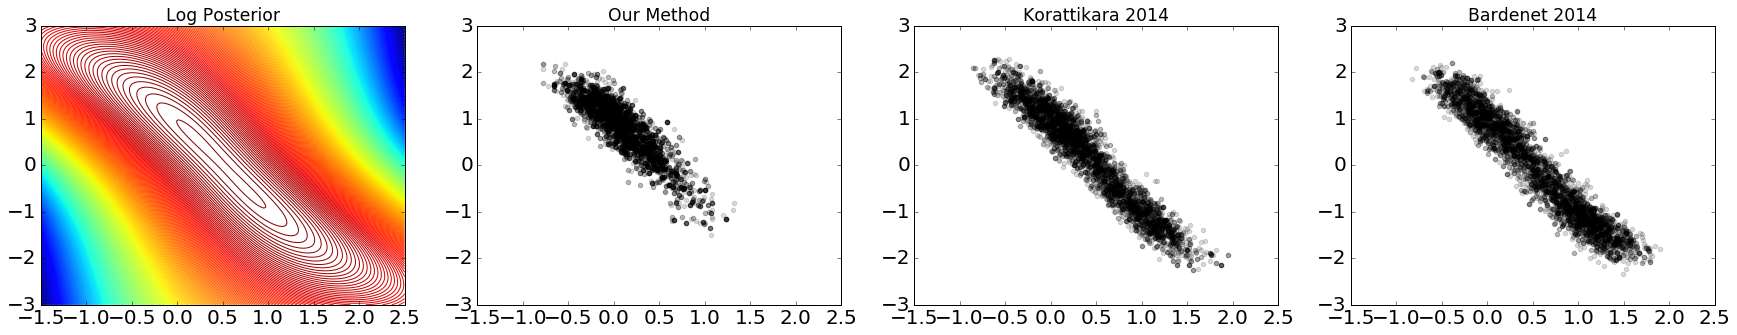
\includegraphics[width=0.9\linewidth]{GaussianMixtureResult/posterior_of_gaussian.png}
    \caption{
    The log posterior contours and scatter plots of sampled $\theta$ values
    using different methods. 
    }
    \label{fig:gauss_mix_1}
\end{figure*}
\begin{figure*}[t]
    \centering
    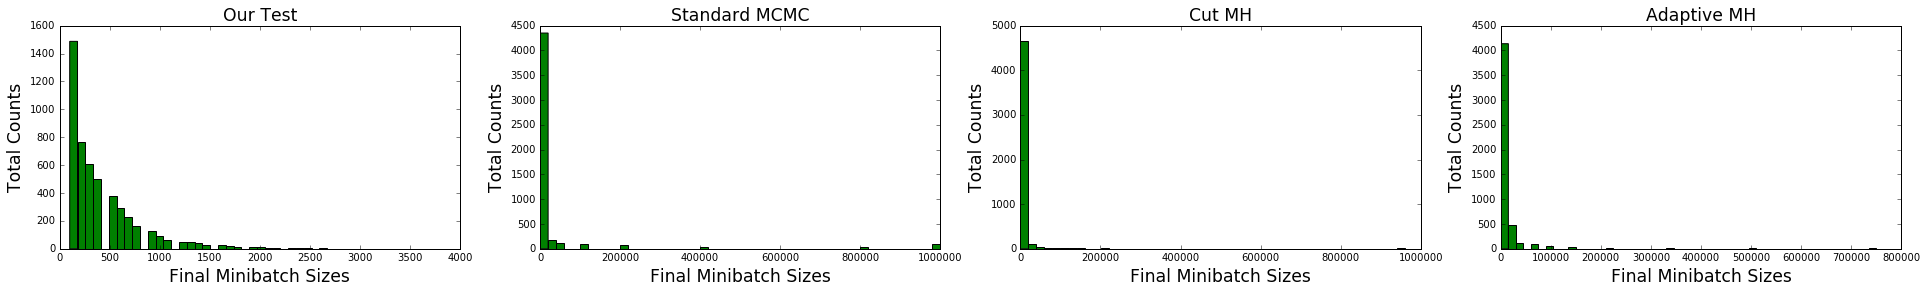
\includegraphics[width=0.9\linewidth]{minibatch_size_gaussian.png}
    \caption{
    Counts of minibatch sizes that the three methods used in the experiment of
    Section~\ref{ssec:gaussians}. To make comparisons easier, the axes have the
    same range (using a log-log scale).
    }
    \label{fig:gauss_mix_2}
\end{figure*}

Figure~\ref{fig:gauss_mix_1} shows scatter plots of the resulting $\theta$
samples for the three methods, with darker regions indicating a greater density
of points. There are no obvious differences, so to better understand any
differences, we measure the similarity between each set of samples and the
actual posterior. 

To effect the comparison, we first discretize the posterior coordinates into
bins (non-overlapping ranges) with respect to the two components of the
parameter $\theta$.  The probability of a sample falling into one of these bins
is the integral of the true posterior probability over the area of that bin. Let
this probability be denoted $P_i$ where $i$ is the bin number. A single sample
from any of the MH methods should therefore be multinomial with distribution
$P$, and a set of $n$ (ideally independent) samples should follow a ${\rm
Multinomial}(P,n)$ distribution.  Since the ideal distribution is simple, we can
use it to measure the quality of the sample distributions rather than use
general purpose tests like KL-divergence or likelihood-ratio.  The latter in any
case are problematic with zero counts in some bins as we have here.

In practice, it is difficult to compute multinomial probabilities for large $n$,
in that case the per-bin distributions are well-approximated by Poisson
distributions with parameter $\lambda_i=P_i n$. Given a set of samples
$\{\theta_1,\ldots,\theta_T\}$, let $c_j$ denote the number of individual samples
$\theta_i$ that fall in bin $j$ out of $N_{\rm bins}$ total. Then we have
\begin{equation}\label{eq:log_prob_poissons}
\begin{split}
    \log p(c_1, \ldots, c_{N_{\rm bins}} \mid P_1, \ldots, P_{N_{\rm bins}}) & =  \\
    \sum_{j=1}^{N_{\rm bins}} c_j \log (n P_j) - n P_j - \log(\Gamma(c_j+1)). & \\
\end{split}
\end{equation}
The results for each model are shown in Table~\ref{tab:poissons}.

While the Poisson results provide general guidance on the relative accuracy of
the models, it is difficult to interpret the quantitative scores. We therefore
perform significance tests to show the difference between the MCMC-sampled
distributions and the ground-truth.  We perform an approximate test using
the Chi-Squared distribution as the test statistic, which we also show in
Table~\ref{tab:poissons}.

Both the Poisson values and the Chi-Squared test statistic result in similar
conclusions: our method is slightly superior to~\citet{cutting_mh_2014}, but
slightly worse than~\citet{icml2014c1_bardenet14}. We now show, however, that
minibatch size results suggest that our method dominates in terms of speed and
efficiency.

Figure~\ref{fig:gauss_mix_2} shows a histogram of the final minibatch sizes used
by the three methods in each iteration. Our method consumes significantly less
data; most minibatch sizes are smaller than 1000, and the average size is 210.
The other methods occasionally need to consume a large proportion of the
entire data set of one million elements; the average minibatch sizes are 15562
and 16857 for Korattikara 2014 and Bardenet 2014, respectively. The average
minibatch sizes accurately predict the running times of these methods since
all methods have a running time proportional to the total data consumed, with
one caveat: the method of~\citet{icml2014c1_bardenet14} requires a global bound
on the term $C_{\theta,\theta'}$ (see Equation~(\ref{eq:bad_bound})) over the
entire the data set at every iteration in order to calculate the error bound.
This bound must be either computed analytically using properties of the specific
dataset, or it must be checked at each sample if a black-box test is required.
We found that the sample code provided by the authors
of~\citet{icml2014c1_bardenet14} in fact computed this bound explicitly for each
sample generated, i.e. the implementation traversed the entire dataset for each
sample, providing no performance advantage over the complete test. For this
reason, we omitted the time to compute $C_{\theta,\theta'}$ from our
measurements of the running time of the sample implementation
of~\citet{icml2014c1_bardenet14}, and consider only the time to process the
minibatches.

%% In Figure ~\ref{fig:gauss_bardenet}, the value
%% of the first part and second part of equation (9)
%% in~\cite{icml2014c1_bardenet14} is shown with respect to the size of actual
%% minibatch data used. The second part which contains  the $C_{\theta,\theta'}$
%% term is larger than the first part, which means that the second part is
%% non-negligible and has to be calculated at every iteration. This is one of the
%% very time-consuming parts in this method.  {\color{blue} Daniel: I am not sure
%% if we should include this plot. Let me think about it and if we decide to
%% include it I will help rewrite the explanation.}

%% JFC - it would still be interesting to see this comparison, however:
%% (i) its important to include equation (9) and explain what the terms are.
%% (ii) the results dont look right. I wouldnt expect the first term to be
%% so small compared to the second and I'm fairly certain they should cross
%% in the illustrated range. It would be better to include both curves on
%% the same plot. 

\begin{table}[t]
    \caption{Gaussian Mixture Model Statistics}
    \label{tab:poissons}
    \centering
    \resizebox{.45\textwidth}{!}{% <------ Don't forget this %
    \begin{tabular}{l l l l}
    {\bf Metric} & {\bf Ours} & {\bf Korat.'14} & {\bf Barde.'14} \\
    \hline
    Equation~\ref{eq:log_prob_poissons} & -1430.0 & -1578.9 & -1232.7 \\
    Chi-Squared & 3313.9 & 3647.7 & 2444.1 \\
    \end{tabular}% <------ Don't forget this %
   }
\end{table}


\subsection{Logistic Regression}\label{ssec:logistic}

\begin{figure*}[t]
	\centering
	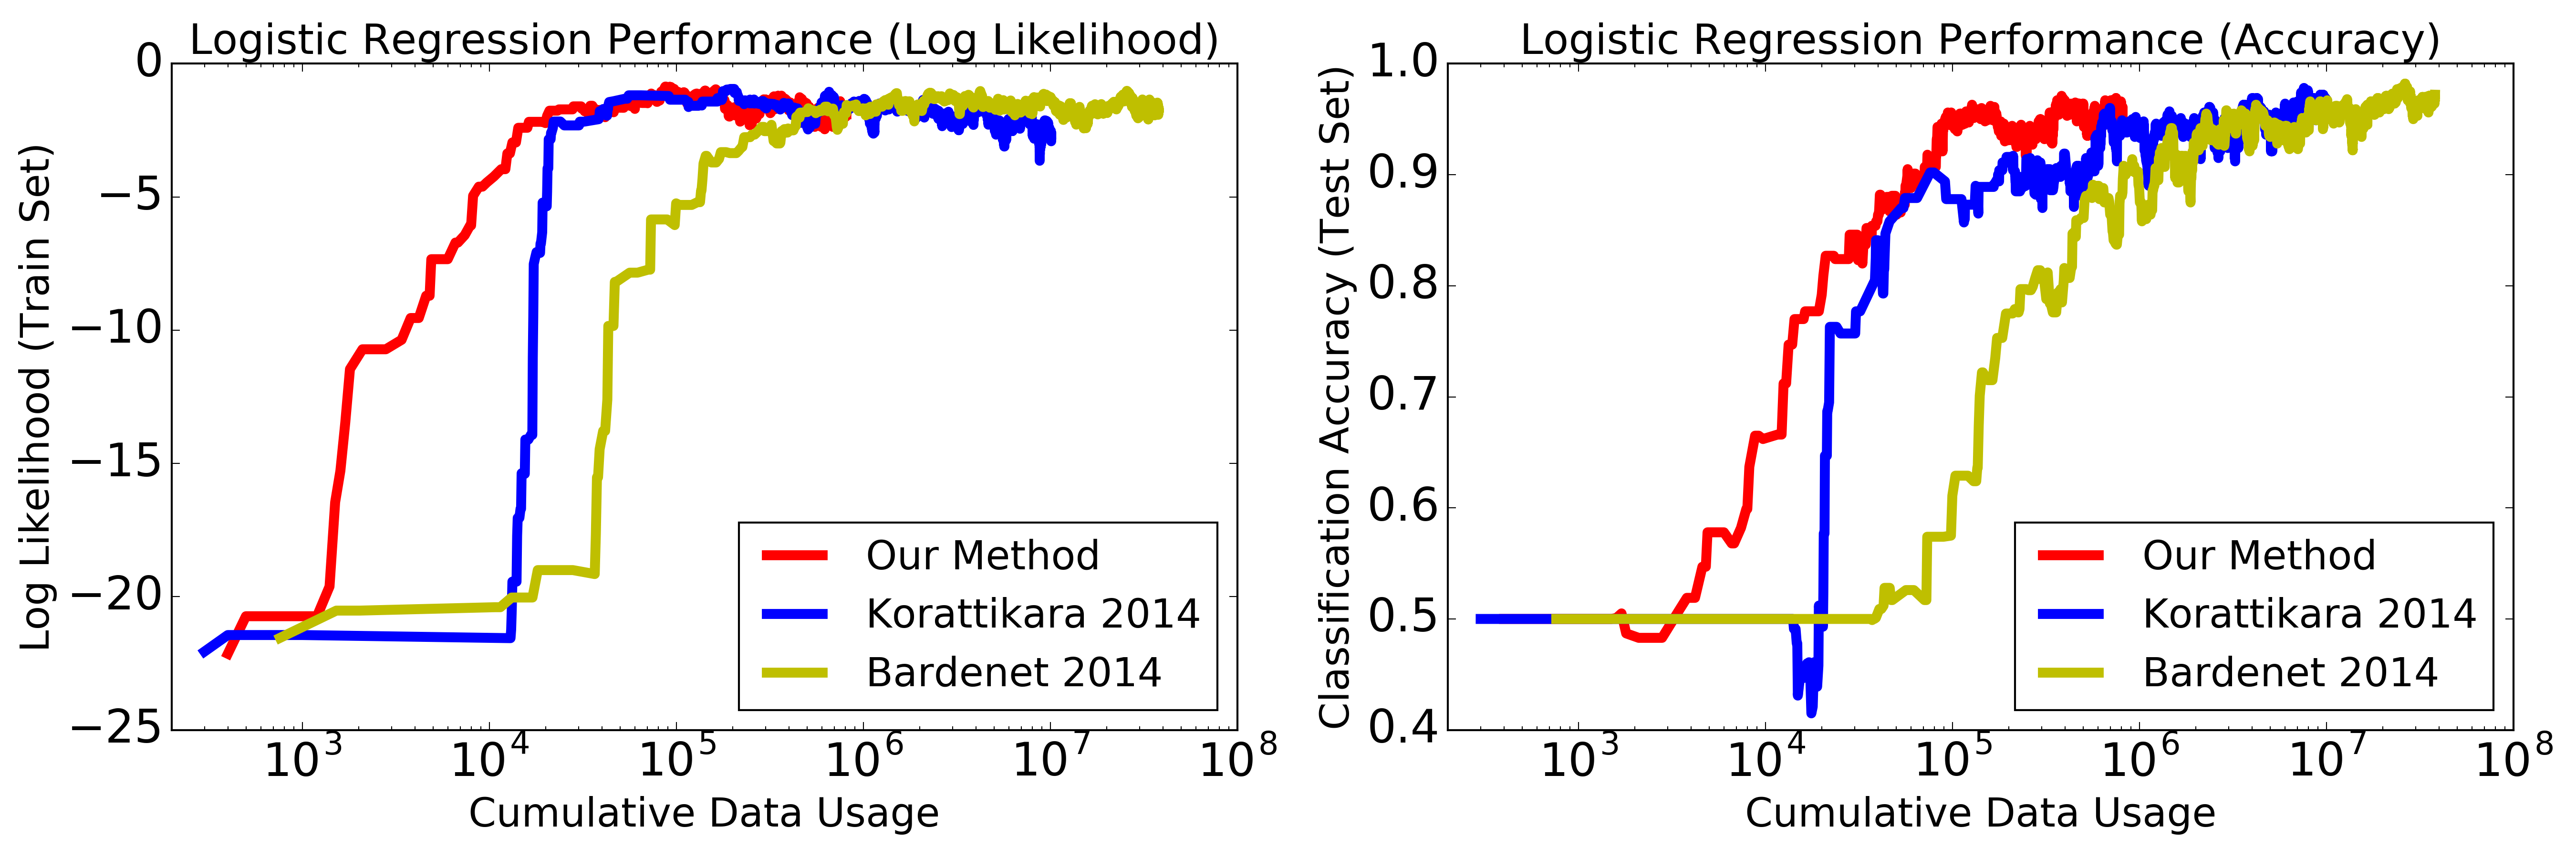
\includegraphics[width=0.9\linewidth]{logistic_performance.png}
	\caption{
    Logistic regression performance (accuracy/log likelihood) based on
    cumulative data usage.
    }
	\label{fig:logistic_performance}
\end{figure*}
\begin{figure*}[t]
	\centering
	\includegraphics[width=0.9\linewidth]{minibatch_size_logistic.png}
	\caption{
    Counts of minibatch sizes that the three methods used in the MNIST logistic
    regression experiment from Section~\ref{ssec:logistic}. It is analogous to
    Figure~\ref{fig:gauss_mix_2}.
    }
	\label{fig:logistic_minibatch}
\end{figure*}

We next use logistic regression for the binary classification of 1s versus 7s in
the MNIST dataset~\citep{lecun-mnisthandwrittendigit-2010}. The data has 12007
training and 1000 testing elements (we used a random subset of the test data).
The pixel values are scaled to be in $(0,1)$.  We impose a flat prior on
$\theta$. For the proposer, we again use a random walk, this time with
covariance matrix $0.05I$ for the $784\times 784$ identity matrix $I$. The
posterior temperature is set at $T=1000$.  We run our MH test and compare with
Korattikara 2014 and Bardenet 2014; minibatch sizes and other parameters are set
to be the same value as with the Gaussian Mixtures experiment from
Section~\ref{ssec:gaussians}.

Figure~\ref{fig:logistic_performance} shows the training log likelihood and the
testing prediction accuracy, each as a function of the cumulative training data
points processed.\footnote{Note that the curves do not span the same length over
the x-axis, because our test consumes fewer samples throughout the MCMC
procedure, so the corresponding curve will ``end'' before the other two.} To
generate the curves, for each of the 5000 sampled vectors $\theta_t$,
$t\in\{1,\ldots,5000\}$, we use $\theta_t$ as the parameter for logistic
regression.  We see that our minibatch MH test is more efficient compared to the
other two methods, because it achieves similar or superior performance while
consuming fewer data points.

Figure~\ref{fig:logistic_minibatch}, in a similar manner as
Figure~\ref{fig:gauss_mix_2}, shows the histogram of minibatch sizes for all
three methods on a log-log scale. With an initial minibatch size of 100,
Korattikara 2014 and Bardenet 2014 achieve average minibatch size of 2026 and
7612 respectively over the MNIST classification task, while our method achieves
that of 163, showing significantly better performance than the benchmark test
methods.



\section{CONCLUSIONS}\label{sec:conclusion}

In this paper, we have derived a new MH test for minibatch MCMC methods. We
demonstrated how a simple deconvolution process allows us to use a minibatch
approximation to the full data tests. We experimentally show the benefits of our
test on Gaussian mixtures and logistic regression.  Straightforward directions
for future work include running more experiments with a particular focus on
investigation of the variance precondition.  More elaborate extensions include
testing on deep neural networks and combining our results with Hamiltonian Monte
Carlo methods, providing a recipe for how to use our algorithm (following the
framework of~\citet{sgmcmc_2015}), or integrating parallel
MCMC~\citep{conf/uai/AngelinoKWSA14,conf/icml/AhnSW14} concepts.





\iffalse
\subsubsection{Figures}

All artwork must be centered, neat, clean, and legible.  All lines
should be very dark for purposes of reproduction, and art work should
not be hand-drawn.  Figures may appear at the top of a column, at the
top of a page spanning multiple columns, inline within a column, or
with text wrapped around them, but the figure number and caption
always appear immediately below the figure.  Leave 2 line spaces
between the figure and the caption. The figure caption is initial caps
and each figure should be numbered consecutively.

Make sure that the figure caption does not get separated from the
figure. Leave extra white space at the bottom of the page rather than
splitting the figure and figure caption.
\begin{figure}[h]
\vspace{.3in}
\centerline{\fbox{This figure intentionally left non-blank}}
\vspace{.3in}
\caption{Sample Figure Caption}
\end{figure}

\subsubsection{Tables}

All tables must be centered, neat, clean, and legible. Do not use hand-drawn tables. Table number and title always appear above the table.
See Table~\ref{sample-table}.

Use one line space before the table title, one line space after the table title, and one line space after the table. The table title must be
initial caps and each table numbered consecutively.

\begin{table}[h]
\caption{Sample Table Title} \label{sample-table}
\begin{center}
\begin{tabular}{ll}
{\bf PART}  &{\bf DESCRIPTION} \\
\hline \\
Dendrite         &Input terminal \\
Axon             &Output terminal \\
Soma             &Cell body (contains cell nucleus) \\
\end{tabular}
\end{center}
\end{table}

\section{SUPPLEMENTARY MATERIAL}

If you need to include additional appendices during submission, you
can include them in the supplementary material file.

\fi


\newpage
\subsubsection*{References}
% Daniel: Sorry, I don't know why this is needed to get rid of the annoying
% spaces below the "References" text.
\vspace{-20pt} 
%\bibliographystyle{apalike}
\bibliographystyle{abbrvnat}
\setcitestyle{authoryear,open={[},close={]}}
\bibliography{aistats2017}


%%%%%%%%%%%%%%%%%%%%%%%%%%%%%%%%%%%%%
\clearpage
\appendix

\begin{center}
{\Large Supplementary Material}
\end{center}

\section{Proof of Lemma~\ref{lem:worst_case}}\label{app:worst_case_proof}

\begin{comment}

{\color{blue} Daniel: changes I made:

\begin{enumerate}
    \item (Somewhat important) I added slightly more detail on why if we assume
    $Y$ has variance $1/N$, then $Y \in \frac{1}{\sqrt{N}}[0.5,1]$ has
    probability $\Phi(1)-\Phi(0.5)$; note that I'm assuming the positive
    interval only, not the negative one. However, you also made $p_0$ double the
    value of $p_1$. I struggled to understand why, until I realized that you
    used the phrase ``with matching sign.'' So I \emph{think} you meant that
    $\theta'-\theta$ could be either positive or negative, but that $\theta-0.5$
    was restricted in its sign so could be only half its value. Is my thinking
    right?

    \item Changed all occurrences of $\Lambda^*(\theta',\theta)$ to
    $\Lambda^*(\theta,\theta')$, i.e., switched the input ordering.

    \item Originally, $\log u_0$ was defined as
    $N(\Lambda^*(\theta,\theta')-\psi(1,\theta,\theta'))$ but I changed the
    starting definition so it does \emph{not} have a factor of $N$ in its
    definition (because we later get $N$ to appear in a subsequent step).

    \item In addition, $\psi(1,\theta,\theta') = 0$ due to uniform priors and
    symmetric proposals and there didn't seem to be a good enough reason to
    include it in the definition so I deleted it (sometimes it's insightful to
    have a nice form of zero inside, but I didn't see it here).

    \item I added in an ``$E$'' because it seemed like you wanted the ``$u$''
    that would make $\psi(u,\theta,\theta') = \log u =
    E[\Lambda^*(\theta,\theta')]$.

    \item Added more detail for the $\Lambda^*(\theta,\theta') \not\approx
    \psi(u,\theta,\theta')$ part.

    \item (TODO later) After Equation~\ref{eq:accept_test_zero}, we say that
    ``the resulting test with our chosen $u_0$ will never correctly succeed
    [...]'', but I think we should say it will not succeed with high
    probability, because we could select a minibatch of samples such that the
    mean \emph{actually is} different from 0.5 (it depends on the distribution
    of the variable that corresponds to $Y = \frac{1}{b}\sum_{i=1}^b x_i$).

    \item (TODO later) Unfortunately, I am unable to understand why ``the size
    of the range in $u$ is at least $\exp([-2,-1.125])$'', unless the real range
    is $\exp([-2,0])$ (as I think it should be) and you were simply cropping off
    the extra range.

    \item (TODO later) My main confusion now is that I am unable to derive
    Equation~\ref{eq:log_uo_range}, and we may want to clarify the notation used
    when we put two intervals side by side.

    \item (TODO later) I do not understand why after
    Equation~\ref{eq:accept_test_rewritten}, we say that the standard deviation
    of the LHS ``given the interval constraints is at least $0.5/\sqrt{b}$.'' We
    already know that the $X_i$ are iid $\mathcal{N}(\theta = 0.5, 1)$ variables
    with a fixed $\theta = 0.5$ value, so we already know the standard deviation
    is supposed to be $\sqrt{({\rm Var}(x_1) + \cdots + {\rm Var}(x_b))/b^2} =
    1/\sqrt{b}$. 

    \item I added Equation~\ref{eq:rhs_range}, which I think is how you
    determined the range. Note that it doesn't seem to matter whether it is
    $[-1,0.75]$ or $[-0.75,1]$ since the main thing that matters is that we have
    maximum absolute value of one.

    \item At the end, it said the joint distribution of
    $(\theta,\theta'-\theta,u)$, but I changed it to $(\theta,\theta',u)$, based
    on your change to the text of Lemma~\ref{lem:worst_case}. But here's a
    question: how is the sample of $\theta'$ (or even $\theta'-\theta$, as it
    was written earlier) independent of $\theta$?
\end{enumerate}
}

\end{comment}

Choose $(\theta' - \theta) \in \pm\frac{1}{\sqrt{N}}[0.5,1]$ (event 1) and $(\theta -0.5)
\in \pm\frac{1}{\sqrt{N}}[0.5,1]$ filtered for  matching sign (event 2).  As
discussed in Lemma~\ref{lem:worst_case}, both $q(\theta' \mid \theta)$ and
$p(\theta \mid x_1,\ldots,x_N)$ have variance $1/N$. If we denote $\Phi$ as the
CDF of the standard normal distribution, then the former event occurs with
probability $p_0 = 2(\Phi(\sqrt{N}\frac{1}{\sqrt{N}}) -
\Phi(\sqrt{N}\frac{0.5}{\sqrt{N}})) = 2(\Phi(1)-\Phi(0.5)) \approx 0.2997$. The
latter event, because we restrict signs, occurs with probability $p_1 =
\Phi(1) - \Phi(0.5) \approx 0.14988$. 

These events together guarantee that $\Lambda^*(\theta,\theta')$ is negative
by inspection of equation (\ref{eq:whyneg}) below.
This implies that we can find a $u \in (0,1)$ so that
$\psi(u,\theta,\theta') = \log u < 0$ equals $E[\Lambda^*(\theta,\theta')]$.
Specifically, choose $u_0$ to satisfy $\log u_0 = E[\Lambda^*(\theta,\theta')]$.
Using $E[x_i] = 0.5$ and Equation~(\ref{eq:lemma_ll_ratio}), we see that
\begin{equation}
  \log u_0 = N(\theta'-\theta)\frac{1}{b} \cdot E\left[\sum_{i=1}^b x_i-\theta-\frac{\theta'-\theta}{2}\right]
\end{equation}
\begin{equation}\label{eq:whyneg}
    \log u_0 = -N(\theta'-\theta)\left(\theta-0.5+\frac{\theta'-\theta}{2}\right).
\end{equation}
Next, consider the minibatch acceptance test $\Lambda^*(\theta,\theta') \not\approx
\psi(u,\theta,\theta')$ used in ~\cite{cutting_mh_2014} and~\cite{icml2014c1_bardenet14} , where $\not\approx$
means ``significantly different from'' under the distribution over
samples of $x_i$. This turns out to be
\begin{equation}
\begin{split}
\Lambda^*(\theta,\theta')  \not\approx \psi(u_0,\theta,\theta') & \quad \\
\iff N(\theta'-\theta) \cdot \frac{1}{b}\sum_{i=1}^b x_i-\theta-\frac{\theta'-\theta}{2} & \not\approx \log u_0\\
\iff \frac{1}{b}\sum_{i=1}^b x_i-\left(\theta+\frac{\theta'-\theta}{2} + \frac{\log u_0}{N(\theta'-\theta)}\right) & \not\approx  0 \\
\iff \frac{1}{b}\sum_{i=1}^b x_i-0.5 & \not\approx 0. \label{eq:accept_test_zero}
\end{split}
\end{equation}
Since the $x_i$ have mean 0.5, the resulting test with our chosen $u_0$ will
never correctly succeed and must use all $N$ data points.  Furthermore, if we
sample values of $u$ near enough to $u_0$, the terms in parenthesis will not be
sufficiently different from 0.5 to allow the test to succeed. 
  
The choices above for $\theta$ and $\theta'$ guarantee that
\begin{equation}\label{eq:log_uo_range}
    \log u_0 \in -[0.5,1][0.75,1.5] = [-1.5, -0.375].
\end{equation}
Next, consider the range of $u$ values near $u_0$:
\begin{equation}\label{eq:log_u_range}
    \log u \in \log u_0 + [-0.5,0.375].
\end{equation}
The size of the range in $u$ is at least $\exp([-2,-1.125]) \approx
[0.13534,0.32465]$ and occurs with probability at least $p_2=0.18932$. With $u$
in this range, we rewrite the test as:
\begin{equation}\label{eq:accept_test_rewritten}
    \frac{1}{b}\sum_{i=1}^b x_i-0.5 \hspace{0.1in} \not\approx \hspace{0.1in} \frac{\log u/u_0}{N(\theta'-\theta)}
\end{equation}
so that, as in Equation~(\ref{eq:accept_test_zero}), the LHS has expected value
zero.  Given our choice of intervals for the variables, we can compute the range
for the right hand side (RHS) assuming\footnote{If $\theta'-\theta<0$, then the
range would be $\frac{1}{\sqrt{N}}[-0.75,1]$ but this does not matter for
the purposes of our analysis.} that $\theta'-\theta > 0$:
\begin{equation}\label{eq:rhs_range}
\begin{split}
    \min\{{\rm RHS}\} & = \frac{-0.5}{\sqrt{N} \cdot 0.5} = -\frac{1}{\sqrt{N}} \\
    {\rm and} \quad \max\{{\rm RHS}\} & = \frac{0.375}{\sqrt{N} \cdot 0.5} = \frac{0.75}{\sqrt{N}}
\end{split}
\end{equation}
Thus, the RHS is in $\frac{1}{\sqrt{N}}[-1,0.75]$.  The standard deviation of
the LHS given the interval constraints is at least $0.5/\sqrt{b}$.
Consequently, the gap between the LHS and RHS in
Equation~(\ref{eq:accept_test_rewritten}) is at most $2\sqrt{b/N}$ standard
deviations, limiting the range in which the test will be able to ``succeed''
without requiring more samples.

The samples $\theta$, $\theta'$ and $u$ are drawn independently and so the
probability of the conjunction of these events is $c = p_0 p_1 p_2 = 0.0085$.

\end{document}
